\section{Z3}\label{Z3}
\subsection{What is Z3}
Z3 is a a theorem prover \cite{z3}. It came in handy with our project, since it can be exploited to solve problems that requires the definition of constraints.\\
In particular, Z3, is composed of two components:
\begin{enumerate}
  \item the \textit{OptSMT} module that is used to solve problems regarding the optimization of classical linear arithmetic objective functions (e.g. Knapsack problem \cite{knapsack});
  \item the \textit{MaxSMT} (actually a collection of \underline{MaxSAT} solvers) module that we're most interested in, because it allows the definition of soft contraints in order to evaluate a solution.
\end{enumerate}

% --------------------------------------------------------------------------

\subsection{Setup of Z3 in machine running Ubuntu}
The development enviroment that has been used is \textbf{Ubuntu}. In order to use Z3 library in such operating system, there are a couple of steps one has to follow.
\begin{enumerate}
  \item \underline{download} the prebuilt version of the library from the offical GitHub repository \url{https://github.com/Z3Prover/z3/releases};
  \item once extracted the files, we have to place them in a specific location in which we will command other applications to look for the needed classes;
  \begin{figure}[!htb]
     \centering
     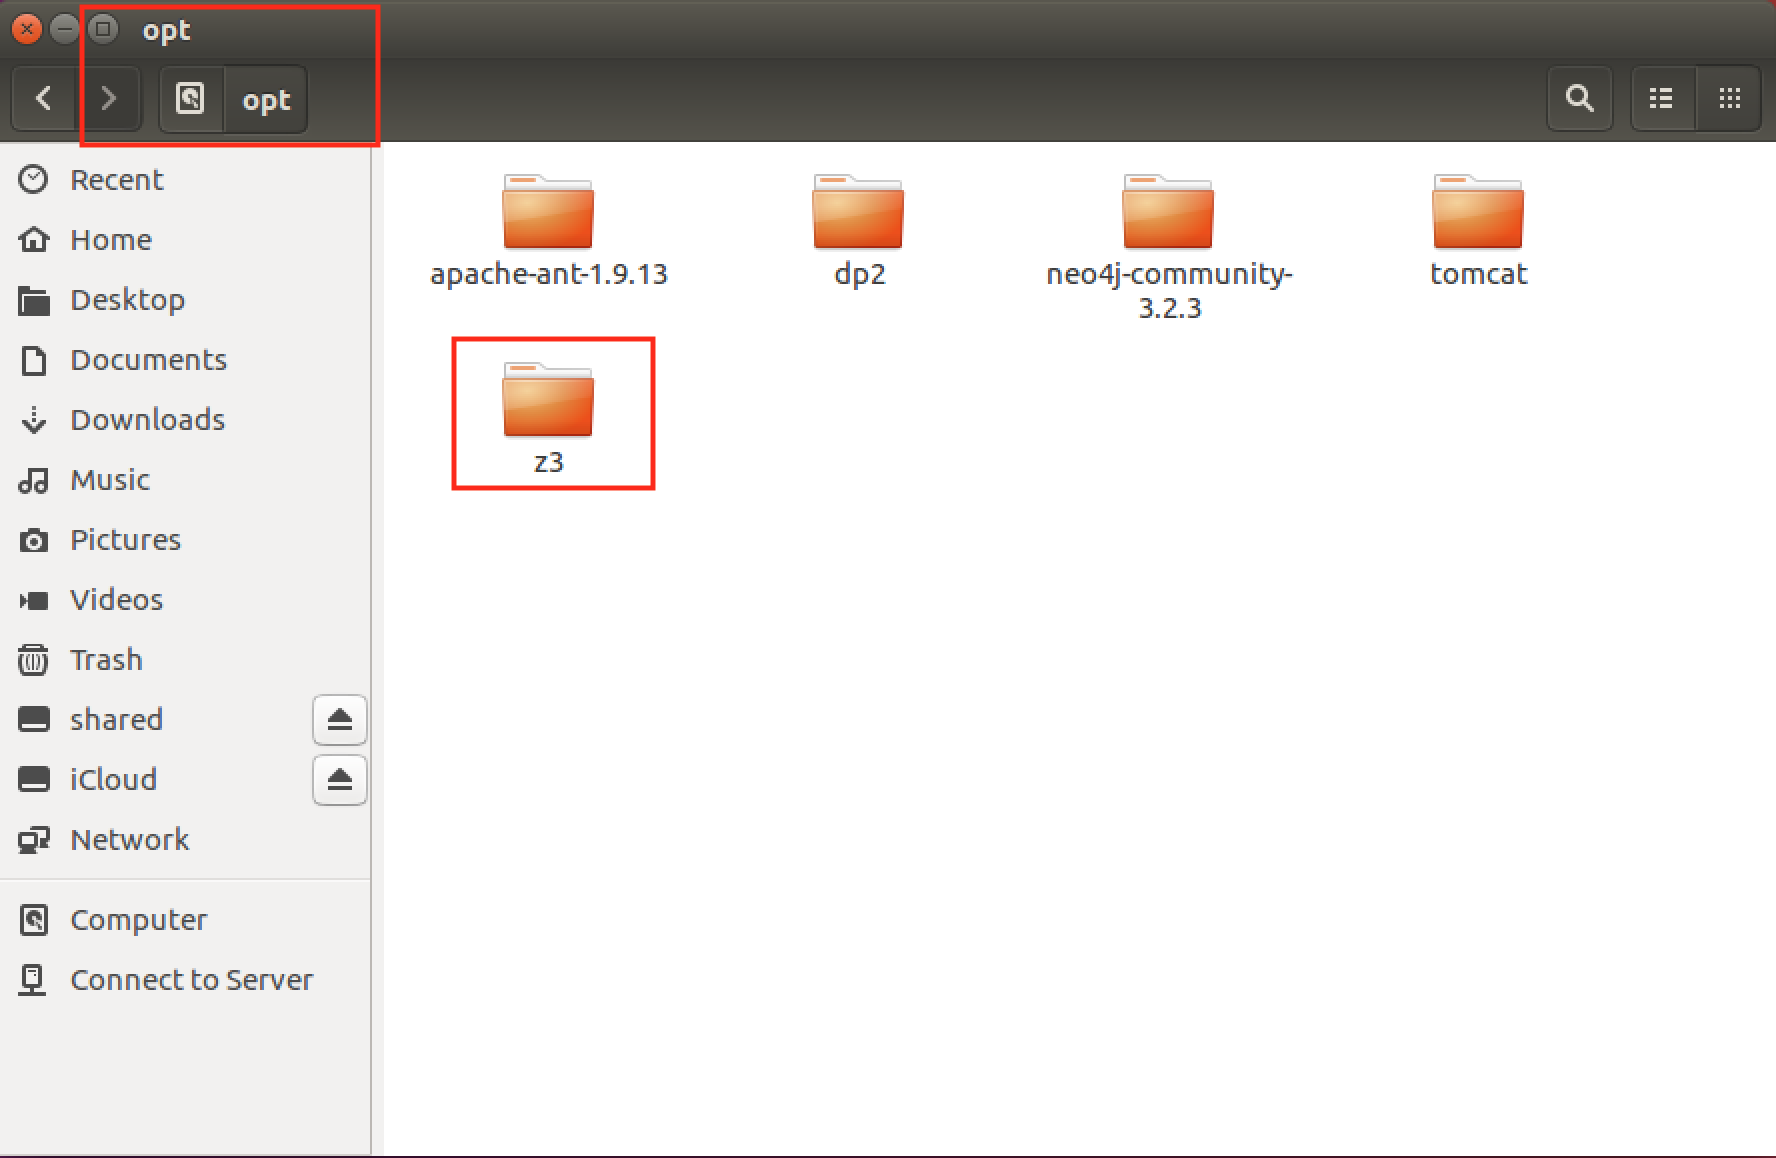
\includegraphics[width=\textwidth]{z3_location.png}
     \caption{Example of where to place Z3 extracted libraries.}\label{Fig:Z3Location}
  \end{figure}
  \item after everything has been placed in the chosen location, we have to \textbf{define} an environment variable which will allow the Java application to know where the Z3 library is located. For Ubuntu such variable is \underline{LD\_LIBRARY\_PATH}. This variable must point to the location of the \underline{bin} folder of the extracted Z3 library;
  \begin{figure}[!htb]
     \centering
     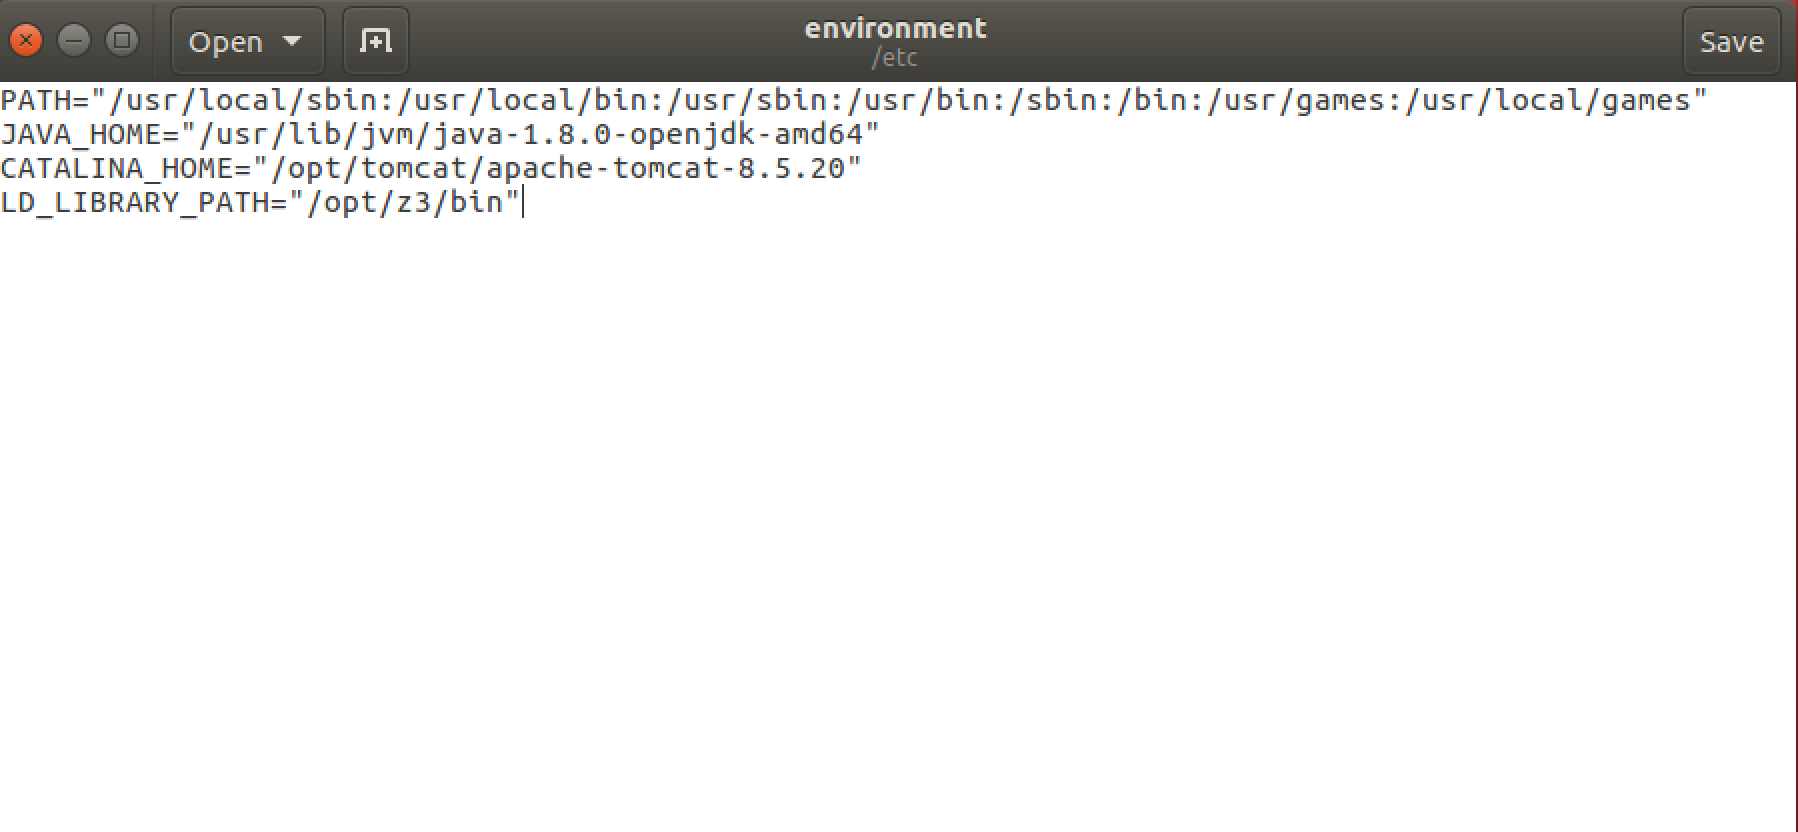
\includegraphics[width=\textwidth]{z3_environment.png}
     \caption{Example of how to define LD\_LIBRARY\_PATH environment variable.}\label{Fig:Z3Environment}
  \end{figure}
  In figure \ref{Fig:Z3Environment} is shown an example of definition of the LD\_LIBRARY\_PATH environment variable. \\
  In this case has been define globally for the whole machine, that means it has been inserted in the file \textit{/etc/environment}, but the same result could have been achieve defining it locally for the used in \textit{/Home/.bashrc} file;
  \item last step, is to add the Z3 .jar file to the build path of our project.
  \begin{figure}[!htb]
     \centering
     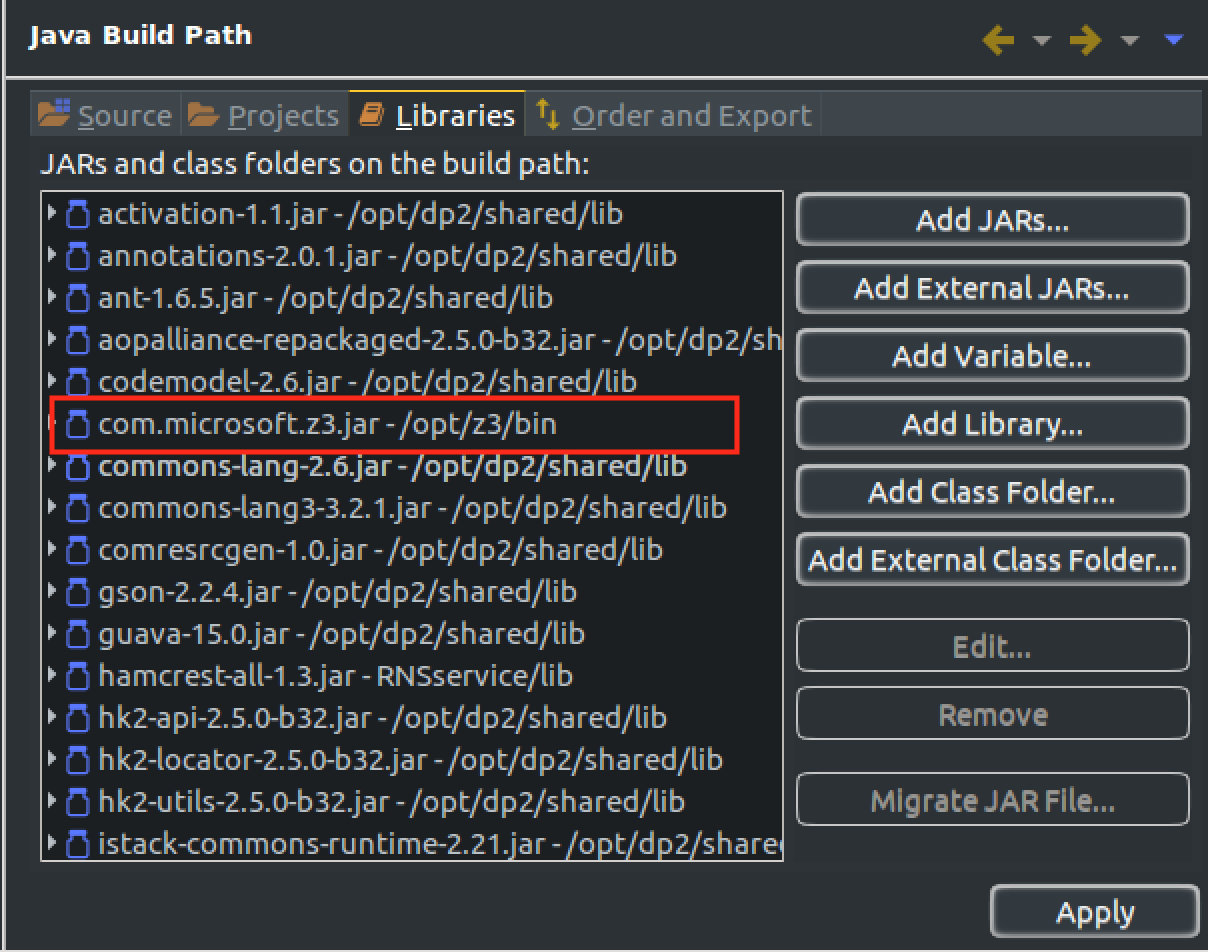
\includegraphics[width=\textwidth]{z3_buildpath.png}
     \caption{Example of how the project build path should look like.}\label{Fig:Z3BuildPath}
  \end{figure}
\end{enumerate}
This is an automatic configuration and Tomcat will load the dynamic libraries in the bin folder by itself. If this is not sufficient, we need to manually put in the WebContent/WEB-INF/lib/jni the Z3 library and point LD\_LIBRARY\_PATH to that folder.\\
Please make sure, in order to use the library in Tomcat, to have correctly set CATALINA\_HOME variable, pointing to Tomcat folder and JAVA\_HOME variable (provided you have installed Java on the machine).

% --------------------------------------------------------------------------

\subsection{Model}
In order to define a model for Z3 to work on, it has been extracted a graph from the actual map stored in the database. The procedure can be subdivided in various steps:
\begin{enumerate}
  \item creation of a context;
  \item extraction of the viable nodes from the map;
  \item definition of constraints to select correct nodes the vehicle can traverse;
  \item definition of soft constraints.
\end{enumerate}
Since the map in not known in advance, in order to traverse the whole graph has been used \textbf{recursion}.\\
The definition of the context and creation of the optimizer class, has been done as shows code snippet \ref{Snip:Z3Init}.
\begin{lstlisting}[language = Java , frame = trBL, escapeinside={(*@}{@*)}, caption = Initialization of context, captionpos=b, label=Snip:Z3Init]
  ctx = new Context();
  mkOptimize = ctx.mkOptimize();
\end{lstlisting}
The context allows the creation of boolean constants, that are assigned a value from the optimizer during its evaluation of feasibility of the problem (based on constraints that have previously been defined).

\subsubsection{Pruning of nodes from the map}
First step is the one to retrieve the nodes from the database and select the ones which don't contain any material or, if vehicle containing materials are present in that node, they have to be compatible with the one carried by the new vehicle entering the system.\\
After selecting these nodes, it has to be defined a boolean expression for each one of them. Such expression will result \textbf{true} if the node has been selected for the path, \textbf{false} otherwise.\\

\subsubsection{Definition of boolean variables}
In order to define boolean variables for the nodes, some other informations are required:
\begin{itemize}
  \item boolean variable of the previous node we're coming from in recursion. If that is true, the current node, \textbf{may be} taken into the path;
  \item boolean variable of the connection between the previous node and the current one. If it is true, and the previous node as well, then the current node \textbf{is} taken in the path.
\end{itemize}
\begin{lstlisting}[language = Java , frame = trBL, escapeinside={(*@}{@*)}, caption = Definition of a boolean expression, captionpos=b, label=Snip:Z3CurrentNode]
	BoolExpr y_curr = ctx.mkBoolConst("y_" + current.getId());
\end{lstlisting}
The code snippet \ref{Snip:Z3CurrentNode} shows how the boolean variables for the nodes have been defined.\\
Once this has been defined it is necessary to derive a variable to determine whether the connection between the previous node and the current one is taken. This step is shown in the snippet \ref{Snip:Z3Connection}.
\begin{lstlisting}[language = Java , frame = trBL, escapeinside={(*@}{@*)}, caption = Definition of a boolean expression for connection between nodes, captionpos=b, label=Snip:Z3Connection]
  this.connectionsBool.put("z_" + prevId + "_" + current.getId(), ctx.mkAnd(y_prev, y_curr));
\end{lstlisting}
The variable for the connection has been defined as the AND between the boolean variable of the previous node and the current one, so that it will result \textbf{true} only if both are \textbf{true}.\\
Last variable it has to be defined is the one responsible for the capacity constraint. It hasn't been used a \textit{BoolExpr} like in the previous cases for this one, instead an \textit{ArithExpr}. Such variable has been defined as the subtraction between the current capacity of the node and 1 as code snippet \ref{Snip:Z3Capacity} shows. In this way, if the arithmetic result is less than 0, the boolean expression defined for the node has to be forced to false, implying that the node has not to be considered.
\begin{lstlisting}[language = Java , frame = trBL, escapeinside={(*@}{@*)}, caption = Definition of arithmetic expression for capacity constraint, captionpos=b, label=Snip:Z3Capacity]
  ArithExpr leftSide = ctx.mkSub(ctx.mkInt(actualCapacity), ctx.mkInt(1));
\end{lstlisting}

\subsubsection{Definition of hard constraints}
Once everything has been created and initialized, it is necessary to specify to the optimizer the policies to assign value (true or false) to the different created variables.\\
First of all the constraint on the capacity has to be defined. This is done the way code snippet \ref{Snip:Z3CapacityConstr} shows.
\begin{lstlisting}[language = Java , frame = trBL, escapeinside={(*@}{@*)}, caption = Definition of capacity constraint for the optimizer, captionpos=b, label=Snip:Z3CapacityConstr]
  ArithExpr capacity = this.nodesCapacity.get(node.getKey());
  mkOptimize.Add(ctx.mkImplies(ctx.mkLt(capacity, ctx.mkInt(0)), ctx.mkNot(node.getValue())));
\end{lstlisting}
In order words if \textit{capacity} is Less Than 0, we force to negate the boolean expression of the node.\\
Then the conditions for the nodes have to be defined:
\begin{itemize}
  \item if the node is the \underline{source} from which the path has to be started, then it has to be true. Since it has no incoming connection from previous nodes (by being the first one), no other constraints have to be defined \ref{Snip:Z3FirstNode};
  \begin{lstlisting}[language = Java , frame = trBL, escapeinside={(*@}{@*)}, caption = Defintion of constraint for the source node, captionpos=b, label=Snip:Z3FirstNode]
    mkOptimize.Add(ctx.mkEq(node.getValue(), ctx.mkBool(true)));
  \end{lstlisting}
  \item if the node is the \underline{destination} of the vehicle, then it has to be true, and it has to have only one incoming connection. No outgoing connection because it is the last node to be visited \ref{Snip:Z3LastNode};
  \begin{lstlisting}[language = Java, frame = trBL, escapeinside={(*@}{@*)}, caption = Defintion of constraint for the destination node, captionpos=b, label=Snip:Z3LastNode]
    mkOptimize.Add(ctx.mkEq(node.getValue(), ctx.mkBool(true)));
    mkOptimize.Add(ctx.mkImplies(node.getValue(), ctx.mkAtLeast(conns.stream().toArray(BoolExpr[]::new), 1)));
    mkOptimize.Add(ctx.mkImplies(node.getValue(), ctx.mkAtMost(conns.stream().toArray(BoolExpr[]::new), 1)));
  \end{lstlisting}
  The node boolean value has to be forced to \textbf{true}, like in the source node case. Since it is true, exactly one (combination of at least one constraint and at most one constraint) connection between all incoming connection (conns is a list containing all the boolean variables for the connection incoming define like in code snippet \ref{Snip:Z3Connection}) has to be selected;
  \item if it is a generic node it has to be inferred that if this node has been selected (boolean variable of the node set to \textbf{true}), then one incoming connection has to be selected as shown in code snippet \ref{Snip:Z3GenericNode}.
  \begin{lstlisting}[language = Java , frame = trBL, escapeinside={(*@}{@*)}, caption = Defintion of constraint for a geneeric node, captionpos=b, label=Snip:Z3GenericNode]
    mkOptimize.Add(ctx.mkImplies(node.getValue(), ctx.mkOr(conns.stream().toArray(BoolExpr[]::new))));
  \end{lstlisting}
  The selection of only two connection per node (one incoming and one outgoing) will be forced by the last node and the definition of soft constraints.
\end{itemize}

\subsubsection{Definition of soft constraints}
The only soft constraint that need to be added to the optimizer is the one on the minimum amount of time predicted for the traversing of the route. This is shown in code snippet \ref{Snip:Z3Soft}
\begin{lstlisting}[language = Java , frame = trBL, escapeinside={(*@}{@*)}, caption = Defintion of soft constraint on minimum traverse time, captionpos=b, label=Snip:Z3Soft]
  for(Entry<String, BoolExpr> node : this.nodes.entrySet()) {
    SimplePlaceReaderType place = Neo4jInteractions.getInstance().getPlace(node.getKey());
    mkOptimize.AssertSoft(ctx.mkNot(node.getValue()), place.getAvgTimeSpent().intValue(), "latency");
  }
\end{lstlisting}
In other words, for each node in the graph, we retrieve information about the place (i.e. average time spent in each place), then we infer that the probability of considering such node in the path is inversely proportional to the average time spent in the node.

\subsubsection{Final result}
The final model from the graph is very simple, only a set of boolean variables representing each one a node in the graph. If the value is \textbf{true}, that means that the node is to be considered in the path, otherwise not.\\
In the snippet \ref{Snip:Z3Model} there is an example for a path evaluated for a newly entered vehicle.
\begin{lstlisting}[frame = trBL , escapeinside={(*@}{@*)}, caption = Final result that need to be parsed to retrieve ne node ids, captionpos=b, label=Snip:Z3Model]
(define-fun y_a02-01 () Bool true)
(define-fun y_ss02 () Bool true)
(define-fun y_a02-02 () Bool false)
(define-fun y_ss01 () Bool false)
(define-fun y_a01-01 () Bool false)
(define-fun y_a01-02 () Bool true)
(define-fun y_a01-03 () Bool false)
(define-fun y_ss03 () Bool true)
(define-fun y_g05 () Bool true)
(define-fun y_g04 () Bool true)
\end{lstlisting}

% --------------------------------------------------------------------------
\subsection{Example}
In this subsection will be presented an example of how the server will compute the correct path for a new vehicle that wants to enter the system.
\begin{figure}[!htb]
   \centering
   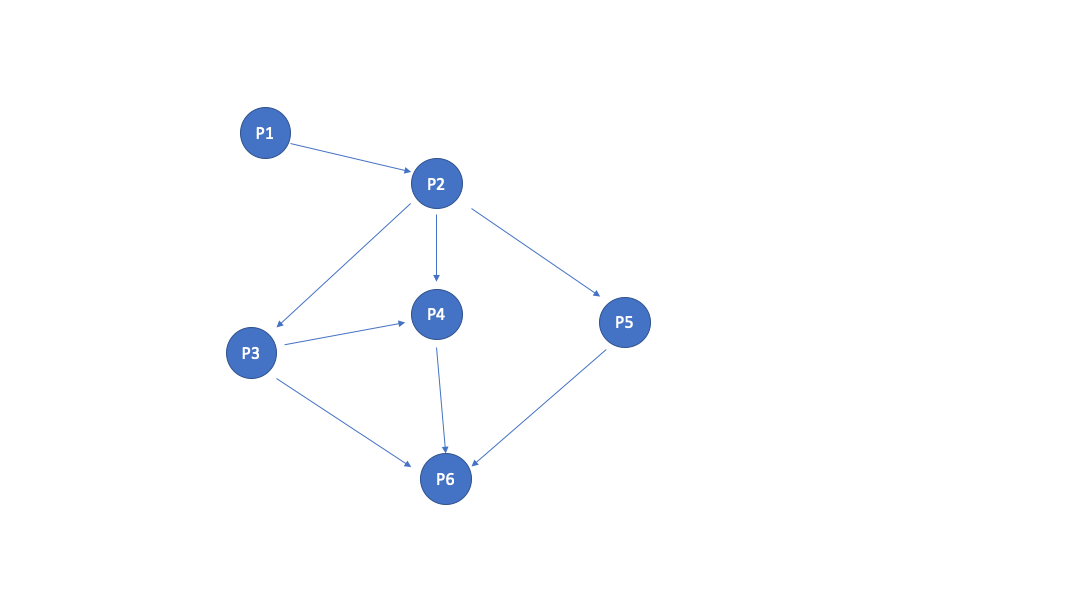
\includegraphics[width=\textwidth]{graph00.png}
   \caption{Example graph.}\label{Fig:Graph00}
\end{figure}
The initial graph that is given Z3 to work on is the one in figure \ref{Fig:Graph00}. Here two assumptions are made:
\begin{enumerate}
  \item node \textbf{P5} contains a vehicle that carries a dangerous material not compatible with the one carried by the new vehicle that wants to enter;
  \item node \textbf{P4} has not enough capacity to accept another vehicle.
\end{enumerate}
The first step that it has to be performed is selecting the origin and destination in the graph (in this case \textbf{P1} and \textbf{P6}) and infer in Z3's optimizer an hard constraint that state that both these nodes has to result \textbf{true} in order to verify the correctness of the solution. The selection of origin node (red) and destination node (green) is shown in fugire \ref{Fig:Graph01}.
\begin{figure}[!htb]
   \centering
   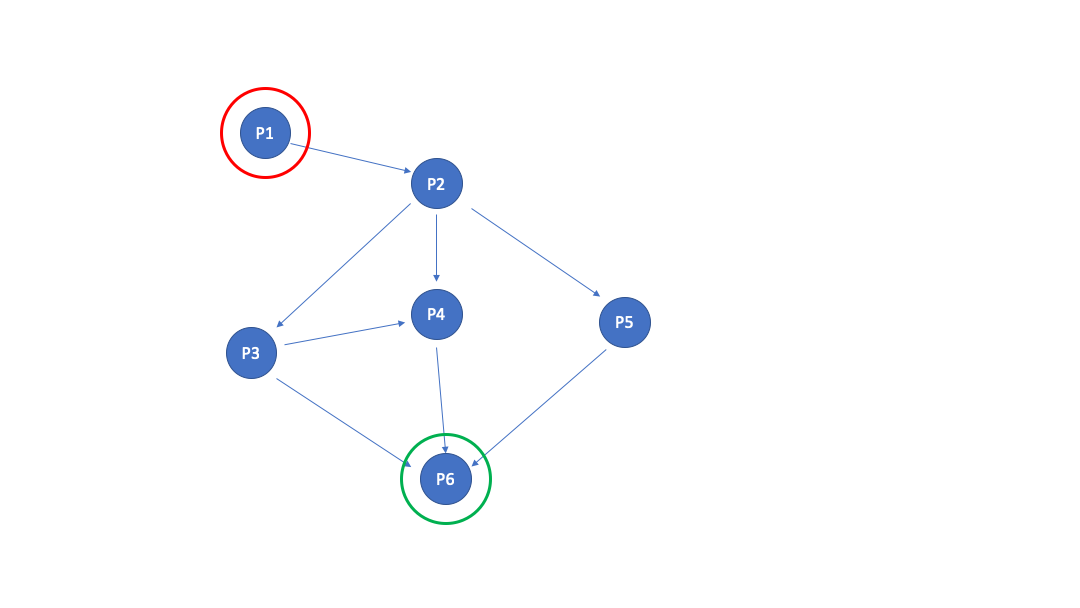
\includegraphics[width=\textwidth]{graph01.png}
   \caption{Selection of origin (red) and destination (green).}\label{Fig:Graph01}
\end{figure}
The next step is pruning from the actual graph, in order to input a correct map to Z3, all the nodes that don't meet the dangerous material constraint. Such constraint states that for a node to be selected it has not to contain any vehicle carrying materials not compatible with the one carried by the vehicle that wants to enter the system. Coherently with assumptions, node \textbf{P5} is pruned out from the graph, since it contains a vehicle with materials not compatible with the new entering (figure \ref{Fig:Graph02}).
\begin{figure}[!htb]
   \centering
   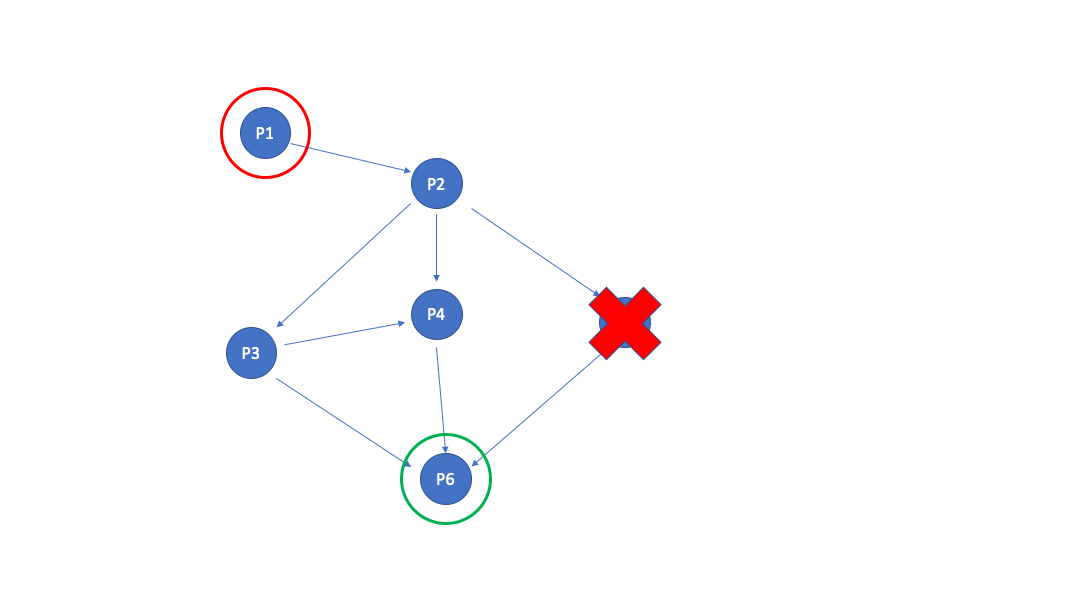
\includegraphics[width=\textwidth]{graph02.png}
   \caption{Pruning of a node due to dangerous materials constraints.}\label{Fig:Graph02}
\end{figure}
Once a correct graph has been retrieve for Z3, the next phase is to define boolean expressions for the optimizer. To achieve that, it is necessary to recur the whole graph in order to explore every node. For each one of them, different expressions has to be defined:
\begin{itemize}
  \item a boolean expression for understanding if a node is considered in the final path, that will result \textbf{true} only if one of its incoming connection's boolean expression is \textbf{true};
  \item a boolean expression for the capacity of the node, that will result to true only if the capacity of the node is greater or equal than 1. If this expression is false, it will invalidate the node as a whole, making it not suitable for the route;
  \item a boolean expression for each one the connection betwee the node and the previous ones. This is not an actual boolean expression, because it is derived from the AND between the two boolean expressions of the nodes at the end of the connection.
\end{itemize}
\begin{figure}[!htb]
   \centering
   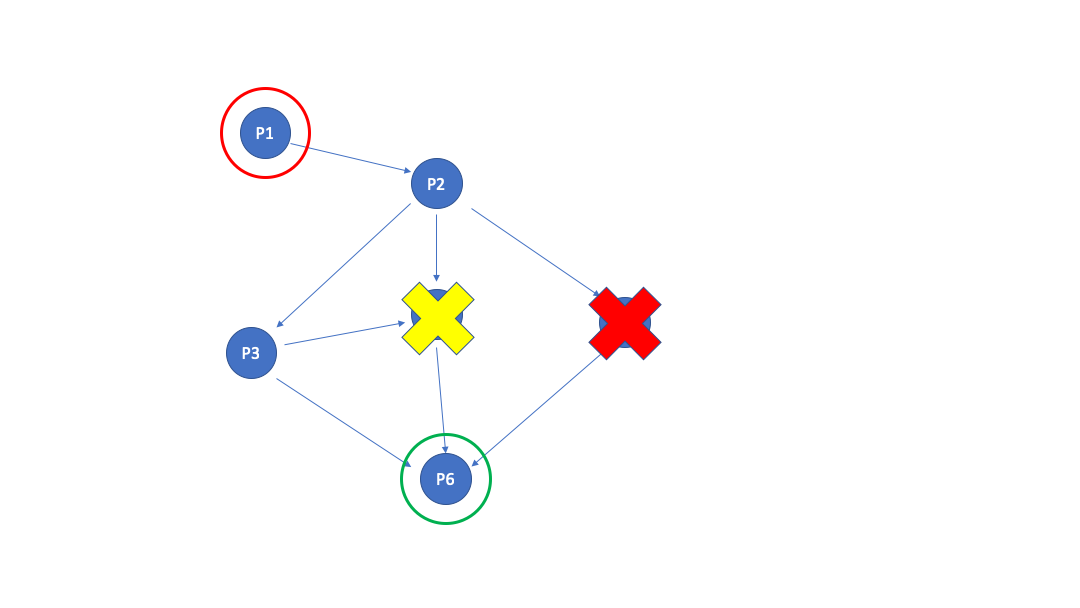
\includegraphics[width=\textwidth]{graph03.png}
   \caption{Pruning of a node due to capacity constraints.}\label{Fig:Graph03}
\end{figure}
Given the definition of such expressions, since the capacity of node \textbf{P4} doesn't meet the requirements as specified above, the corresponding boolean expression of the node is invalidated by the optimized, making it not a suitable node for the evaluation of a path as shown in figure \ref{Fig:Graph03}.
\begin{figure}[!htb]
   \centering
   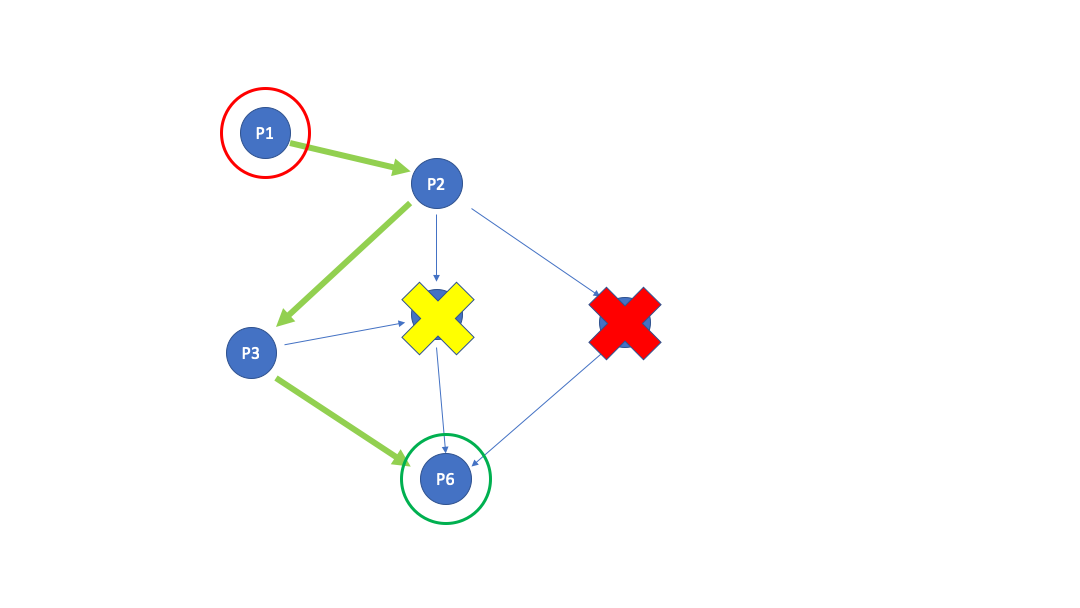
\includegraphics[width=\textwidth]{graph04.png}
   \caption{Evaluation of path from source to destination.}\label{Fig:Graph04}
\end{figure}
The resulting path produced by Z3 is the one show in figure \ref{Fig:Graph04}. In the case multiple paths are present from source to destination, the optimizer will choose the one with the minimum traverse time, using the min time constraint define as subsection \ref{Subs:MathModel} shows.
